% Group 9, Smart HVAC Optimisation: architecture document (D7065E final report).
% Preamble and title block: the course's final_report_template.tex.
% We drafted the report in Markdown and converted it once with pandoc; this file is now the source.
% Diagrams: docs/diagrams/<name>.mmd, drawn to docs/figures/<name>.png by scripts/build_report.py.
% Build: python3 scripts/build_report.py   (or pdflatex D7065E_Group9_Final_Report.tex twice, from docs/)
\PassOptionsToPackage{unicode}{hyperref}
\PassOptionsToPackage{hyphens}{url}
\PassOptionsToPackage{dvipsnames,svgnames,x11names}{xcolor}
\documentclass[11pt]{article}
\usepackage{amsmath,amssymb}
\usepackage{lmodern}
\usepackage{iftex}
\ifPDFTeX
  \usepackage[T1]{fontenc}
  \usepackage[utf8]{inputenc}
  \usepackage{textcomp}
\fi
\IfFileExists{microtype.sty}{\usepackage[]{microtype}\UseMicrotypeSet[protrusion]{basicmath}}{}
\makeatletter
\@ifundefined{KOMAClassName}{%
  \IfFileExists{parskip.sty}{\usepackage{parskip}}{%
    \setlength{\parindent}{0pt}\setlength{\parskip}{6pt plus 2pt minus 1pt}}
}{\KOMAoptions{parskip=half}}
\makeatother
\usepackage{xcolor}
\IfFileExists{xurl.sty}{\usepackage{xurl}}{}
\IfFileExists{bookmark.sty}{\usepackage{bookmark}}{\usepackage{hyperref}}
\hypersetup{
  pdftitle={Smart HVAC Optimisation, Architecture Document},
  pdfauthor={Group 9: Monika Shrivastava and Abhay Soni},
  colorlinks=true,
  linkcolor={RoyalBlue},
  filecolor={Maroon},
  citecolor={Blue},
  urlcolor={Blue}}
\urlstyle{same}
\usepackage[a4paper,margin=2.4cm]{geometry}
\usepackage{longtable,booktabs,array}
\makeatletter\@ifundefined{c@none}{\newcounter{none}}{}\makeatother % tables without a caption (pandoc 3)
\usepackage{calc}
\usepackage{graphicx}
\makeatletter
\def\maxwidth{\ifdim\Gin@nat@width>\linewidth\linewidth\else\Gin@nat@width\fi}
\def\maxheight{\ifdim\Gin@nat@height>\textheight\textheight\else\Gin@nat@height\fi}
\def\verbatim@font{\scriptsize\ttfamily}
\makeatother
\setkeys{Gin}{width=\maxwidth,height=\maxheight,keepaspectratio}
\makeatletter % pandoc 3 puts images in \pandocbounded (from pandoc's default template)
\newsavebox\pandoc@box
\newcommand*\pandocbounded[1]{\sbox\pandoc@box{#1}%
  \Gscale@div\@tempa{\textheight}{\dimexpr\ht\pandoc@box+\dp\pandoc@box\relax}%
  \Gscale@div\@tempb{\linewidth}{\wd\pandoc@box}%
  \ifdim\@tempb\p@<\@tempa\p@\let\@tempa\@tempb\fi
  \ifdim\@tempa\p@<\p@\scalebox{\@tempa}{\usebox\pandoc@box}\else\usebox{\pandoc@box}\fi}
\makeatother
\setlength{\emergencystretch}{3em}
\providecommand{\tightlist}{\setlength{\itemsep}{0pt}\setlength{\parskip}{0pt}}
\setcounter{secnumdepth}{-\maxdimen}
\usepackage{newunicodechar}
\usepackage{textcomp}
\usepackage{amssymb}
\newunicodechar{°}{\textdegree}
\newunicodechar{₂}{\textsubscript{2}}
\newunicodechar{→}{\ensuremath{\rightarrow}}
\newunicodechar{≤}{\ensuremath{\leq}}
\newunicodechar{≥}{\ensuremath{\geq}}
\newunicodechar{≈}{\ensuremath{\approx}}
\newunicodechar{✓}{\ensuremath{\checkmark}}
\newunicodechar{–}{--}
\newunicodechar{—}{---}
\newunicodechar{²}{\textsuperscript{2}}
\newunicodechar{³}{\textsuperscript{3}}
\newunicodechar{·}{\ensuremath{\cdot}}
\newunicodechar{×}{\ensuremath{\times}}
\newunicodechar{−}{\ensuremath{-}}
\newunicodechar{…}{\ldots}
\newunicodechar{η}{\ensuremath{\eta}}
\newunicodechar{π}{\ensuremath{\pi}}
\newunicodechar{ρ}{\ensuremath{\rho}}
\newunicodechar{⟨}{\ensuremath{\langle}}
\newunicodechar{⟩}{\ensuremath{\rangle}}
\usepackage{etoolbox}
\AtBeginEnvironment{longtable}{\footnotesize}
\AtBeginEnvironment{tabular}{\footnotesize}
\usepackage{fancyhdr}
\pagestyle{fancy}\fancyhf{}
\rhead{\small D7065E\,--\,Architecture Document}
\lhead{\small Group 9: Smart HVAC Optimisation}
\cfoot{\thepage}
\renewcommand{\headrulewidth}{0.4pt}
\usepackage{titlesec}
\titleformat{\section}{\Large\bfseries}{\thesection}{0.6em}{}
\titleformat{\subsection}{\large\bfseries}{\thesubsection}{0.5em}{}
\usepackage{microtype}
\setlength{\emergencystretch}{2em}

\begin{document}

\begin{center}
{\LARGE Smart HVAC Optimisation\par}
\vspace{0.5em}
{\large D7065E, Architecture Document\par}
\vspace{1em}
{Group 9: Monika Shrivastava \& Abhay Soni\par}
\end{center}
\vspace{1.2em}
{
\hypersetup{linkcolor=black}
\setcounter{tocdepth}{3}
\tableofcontents
}
\newpage

% Helpers: column with a width as a fraction of the line, a figure, and a figure caption.
\newcolumntype{L}[1]{>{\raggedright\arraybackslash}p{\dimexpr#1\linewidth-2\tabcolsep\relax}}
\newcommand{\fig}[2]{\begin{center}\includegraphics[width=\linewidth,height=#2\textheight,keepaspectratio]{figures/#1}\end{center}\vspace{-0.8em}}
\newcommand{\figcap}[1]{\par\noindent{\footnotesize\emph{#1}}\par\medskip}

\section{1. Summary}\label{summary}

Our system controls the heating and ventilation of four offices on level 0 of the LTU
A-house. When someone is in an office it keeps the room comfortable and ventilated; when the
office is empty it lowers the temperature and the ventilation; and it learns when people
usually arrive, so it can warm the room before they come. A fixed-schedule controller runs
next to it in two other offices, so the difference can be measured. The building, its
devices and the 3D view come from BuildSim; we built the physics, the sensors, the data
pipeline, the decisions and the evaluation around it. The idea behind every design choice:
\textbf{heat where and when people are, and do not act on data you cannot trust.}

\begin{longtable}{@{}L{0.3}L{0.7}@{}}
\toprule
\textbf{Field} & \textbf{Value} \\
\midrule
\endhead
\bottomrule
\endlastfoot
\textbf{Project title} & Smart HVAC Optimisation \\
\textbf{Team members} & Monika Shrivastava, Abhay Soni \\
\textbf{Use case} & Occupancy-based heating and ventilation of offices \\
\textbf{Repository} & \texttt{github.com/abhay9993/D7065E-project-Group-9} \\
\textbf{Version / date} & Final / 2026-10-12 \\
\end{longtable}

\textbf{Changes since the proposal.} We first built a working prototype of every service and
tested it for a few days. What we saw there led to these changes:
\begin{itemize}
\tightlist
\item \textbf{Physics:} the first room model could not keep rooms warm on a cold day, so we rebuilt
  it as a heat balance with a room heater that has its own thermostat (Section 6).
\item \textbf{Forecast:} a trend over recent occupancy cannot predict an arrival in an empty room, so
  the controller now learns when each room is usually used (Section 7.1).
\item \textbf{Data:} a pipeline restart lost the stored history, so readings are now saved to a file,
  and sensors keep unsent readings until the pipeline is back (Section 7.2).
\item \textbf{Fair comparison:} the first baseline did not use the same clock as the people, so
  everything now runs on one model clock and we compare rooms of similar size (Section 11).
\item \textbf{Rooms:} the occupancy simulator puts one person in every small room, so we compare
  offices instead of the meeting room in the proposal.
\end{itemize}

\section{2. Use case and building context (BuildSim)}\label{use-case}

\textbf{The building.} BuildSim provides the LTU A-house: floor plans, rooms and their areas,
devices with their current values, who is in which room, and a 3D viewer. It does not simulate
or decide anything; it is the shared state of the system. We did not change it, we only read
from it and write to it.

\textbf{How the system connects to BuildSim.} Every collection in BuildSim has exactly one writer:
\begin{itemize}
\tightlist
\item The \textbf{occupancy simulator} (from the course) moves people and writes the occupancy.
\item Our \textbf{physical simulator} reads the occupancy and the actuator state, advances the room
  physics and writes the true sensor values (\texttt{PUT /api/sensors/\{id\}/value}). This is
  where the loop closes.
\item The four \textbf{sensor processes} only read: they sample the values from BuildSim, add
  device noise and send readings to our pipeline.
\item The \textbf{actuator} is the only writer of actuator state
  (\texttt{PUT /api/actuators/\{id\}/state}).
\item The \textbf{dashboard} writes a temperature layer and alerts for the 3D view. The controller,
  the baseline, the pipeline and the evaluation never touch BuildSim.
\end{itemize}

\textbf{Actors.} The building manager watches the dashboard and the 3D view. Occupants only
affect the system by being present; they are sensed, not connected.

\textbf{The scenario the demo tells.} It is 07:45 on a Wednesday. Our controller has learned that
someone usually arrives in A1013 after 08:00, so it warms the room up from the 18 °C night
setback. When the person walks in, the room switches to ``occupied'' within one decision cycle;
during a coffee break it stays warm for 30 minutes. Next door, the fixed schedule heats its
rooms from 07:00 to 18:00 whether anyone is there or not. During the demo we also stop and
crash services to show what happens.

\textbf{Why it matters.} Heating and ventilation use most of the energy in Swedish offices, and
offices are often empty. Following people instead of the clock can save energy, but only if
the rooms stay comfortable, the system reacts fast enough, and it behaves safely when its
data is wrong. Those three concerns drive the requirements.

\textbf{Rooms and time.} We use two size-matched pairs: A1009 (15.3 m², ours) with A1010 (13.8 m²,
schedule), and A1013 (27.2 m², ours) with A1015 (31.3 m², schedule). The occupancy simulator owns
the model clock, which runs 60 times faster than real time (a model day takes 24 real minutes).
Everything about the building (schedules, grace period, learned table, physics) uses model time;
everything about the processes (latency, staleness, recovery) uses real seconds.

\section{3. Requirements}\label{requirements}

Each requirement is a testable statement with a unique ID. It is traced to a test in Section 10
and to a measured result in Section 11.

\begin{longtable}{@{}L{0.1}L{0.12}L{0.25}L{0.1}L{0.23}L{0.2}@{}}
\toprule
\textbf{ID} & \textbf{Type} & \textbf{Requirement} & \textbf{Priority} & \textbf{Acceptance criterion} & \textbf{Verified by} \\
\midrule
\endhead
\bottomrule
\endlastfoot
FR-01 & Functional & When someone is in an office, keep the room inside the comfort band & Must & ≥ 90 \% of occupied time in 20--24 °C (EN 16798-1, category II) & long run \\
FR-02 & Functional & Have the room already comfortable when someone arrives, by heating before their usual arrival time & Should & ≥ 80 \% of the first 30 min after an arrival in 20--24 °C & long run \\
FR-03 & Functional & Turn heating and ventilation down in rooms that are empty and where nobody is expected soon & Must & 18 °C within one decision once a room is empty for 30 min and nobody is expected; never below 17 °C & \texttt{Test\allowbreak{}Empty\allowbreak{}Room\allowbreak{}Sets\allowbreak{}Back\allowbreak{}Unless\allowbreak{}Arrival\allowbreak{}Is\allowbreak{}Likely} \\
FR-04 & Functional & Ventilate more when a room becomes too humid & Should & Humidity > 60 \% gives fan ≥ 80 \% & \texttt{Test\allowbreak{}Humidity\allowbreak{}Raises\allowbreak{}Ventilation\allowbreak{}But\allowbreak{}Is\allowbreak{}Not\allowbreak{}Safety\allowbreak{}Critical} \\
NFR-01 & Non-functional & React to a person arriving within two decision cycles & Must & Arrival sensed → command applied in ≤ 20 s & \texttt{test\_\allowbreak{}e2e} \\
NFR-02 & Non-functional & Recover by itself after a sensor crash or a BuildSim restart & Must & Data and commands flow again ≤ 60 s after a sensor crash or a BuildSim restart & \texttt{test\_\allowbreak{}f1\_\allowbreak{}buildsim\_\allowbreak{}restart} \\
NFR-03 & Non-functional & Lose no sensor readings while the data pipeline is down & Must & A 30 s outage leaves no gap > 7 s in the stored readings & \texttt{test\_\allowbreak{}f2\_\allowbreak{}pipeline\_\allowbreak{}outage} \\
NFR-04 & Non-functional & Use clearly less energy than a fixed office-hours schedule & Should & ≥ 15 \% less kWh per m² over one week & long run \\
NFR-05 & Non-functional & Notice bad sensor data (frozen, old, missing or impossible) and fall back to a safe setting & Must & A stuck, stale or silent sensor gives the safe default in ≤ 90 s; impossible values are rejected & \texttt{test\_\allowbreak{}f4\_\allowbreak{}stuck\_\allowbreak{}temperature} \\
NFR-06 & Non-functional & Keep the rooms safe if a controller stops sending commands & Must & Its rooms get a safe state ≤ 70 s after the last command & \texttt{test\_\allowbreak{}f3\_\allowbreak{}controller\_\allowbreak{}down} \\
NFR-07 & Non-functional & Keep up with a much bigger building and faster updates & Should & Decision cycle ≤ 10 s and simulator tick ≤ 5 s with ≥ 50 rooms & stress test \\
REG-01 & Regulatory & Give occupied rooms enough fresh air, as Swedish work-environment rules require (AFS 2020:1) & Must & Fan ≥ 50 \% while the room is occupied & \texttt{Test\allowbreak{}Occupied\allowbreak{}Room\allowbreak{}Held\allowbreak{}At\allowbreak{}Comfort\allowbreak{}And\allowbreak{}Ventilated} \\
\end{longtable}

{\footnotesize \texttt{test\_\ldots}: system tests; \texttt{Test\ldots}: Go unit tests; the long run and the
stress test are the experiments in Section 11. Section 10 says how each one works.}

\textbf{Tension.} Comfort and fresh air (FR-01, FR-02, REG-01) push heating and ventilation up,
energy (NFR-04) pushes them down, and when the data is bad (NFR-05) neither goal can be trusted,
so the controller falls back to a safe default. Balancing these safely is the controller's job.

\textbf{Traceability.} The requirement names its test here, Section 10 says how each test works
and what evidence it leaves, and Section 11 gives the measured result against the acceptance
criterion.

\section{4. Architecture}\label{architecture}

\subsection{4.1 Context diagram (C4 Level 1)}

\fig{context.png}{0.42}
\figcap{Figure 1. C4 System Context (Level 1). Our system is the blue box; the grey boxes are the
course's systems, which we use but did not change. As in Figure 2, arrows show which way the data
flows.}

The system (Figure 1) reads and changes the building only through BuildSim, and reads the model clock from
the occupancy simulator. Both come from the course and run unchanged in our compose file. The
building manager watches; the occupants are simulated by the occupancy simulator and sensed through BuildSim. No external computer (GPU server or LLM) is used.

\subsection{4.2 Container diagram (C4 Level 2)}

\fig{container.png}{0.55}
\figcap{Figure 2. C4 Container diagram (Level 2). The dashed box is our system: each box in it is one
service in \texttt{docker-compose.yaml} and one folder. Grey boxes are the course's systems. Arrows
show which way the data flows, labelled with the data and the REST call that moves it.}

The loop in Figure 2: the simulator writes the true values into BuildSim; the sensors read them and push
readings to the pipeline; every 10 s the controller asks the pipeline for the room state,
decides, and posts a command to the actuator, which writes it into BuildSim. On its next tick
the simulator reads the new setpoint and fan, the room reacts, and the next reading shows it.
That feedback is what makes this a cyber-physical system rather than a dashboard.


\textbf{Component responsibilities.} Every container has one job, so it can be tested alone and can
fail without taking the rest down.

\begin{longtable}{@{}L{0.15}L{0.26}L{0.19}L{0.08}L{0.32}@{}}
\toprule
\textbf{Component} & \textbf{Responsibility (one job)} & \textbf{Container} & \textbf{Tech} & \textbf{Reason for separation} \\
\midrule
\endhead
\bottomrule
\endlastfoot
Physical simulator & Room physics from occupancy and actuator state & \texttt{simulator} & Go & Plays the building; a real building could replace it \\
Sensors & Sample one kind of value for all rooms, add noise, deliver & \texttt{sensor-*} (4) & Go & A crash loses one kind of value only; one program, run four times \\
Data pipeline & Check, de-duplicate, store, flag stale or stuck data & \texttt{pipeline} & Go & Every consumer gets the same data-quality verdict \\
Controller & Decide setpoint and fan for each room & \texttt{controller} & Go & Decision logic changes most; restart without touching devices \\
Baseline & The same job on a fixed schedule & \texttt{baseline-}\allowbreak\texttt{controller} & Go & Runs at the same time, with the same weather and clock \\
HVAC actuator & Only writer of actuator state: clamp, ownership, lease & \texttt{hvac-actuator} & Go & Nothing unsafe reaches the building, even if a controller dies \\
Evaluation & Measure comfort and energy, check requirements & \texttt{evaluation} & Go & The evidence does not depend on the thing being judged \\
Dashboard & Tables, 3D layer and alerts & \texttt{dashboard} & Go & Can crash or change without affecting control \\
BuildSim, occupancy simulator & Building state; people and the model clock & \texttt{buildsim}, \texttt{occupancy-sim} & Go & Provided by the course, not changed \\
\end{longtable}

\subsection{4.3 Component diagram (C4 Level 3): the controller}

\fig{component.png}{0.3}
\figcap{Figure 3. C4 Component diagram (Level 3) of the controller, the container that makes the
decisions. Grey boxes are the containers and systems it talks to; arrows show the data flow.}

The controller polls the pipeline, reads the model clock and the learned table, and passes all of
it to \texttt{decide()}. That is a plain function: it gets the room state, the time, when the room
was last occupied and the learned probability, and returns the setpoint, fan, mode and a reason. So
every rule can be unit tested without the network. The command goes to the actuator, and every
decision is written to an audit log (Section 7.1).

\subsection{4.4 Design decisions and alternatives}

Each row gives the option we chose, the alternative we rejected, the requirement it serves, and
the price we pay.

\begin{longtable}{@{}L{0.16}L{0.21}L{0.17}L{0.26}L{0.2}@{}}
\toprule
\textbf{Decision} & \textbf{Chosen} & \textbf{Alternatives} & \textbf{Justification (requirement)} & \textbf{Trade-off} \\
\midrule
\endhead
\bottomrule
\endlastfoot
Sensor transport & HTTP to the pipeline; sensors keep and re-send unsent readings & MQTT broker; Kafka & Only the pipeline needs raw readings; the sensor buffer gives no loss in an outage (NFR-03) & Buffer is in memory (1000 readings) \\
Storage & Append-only JSONL file, read back at start; recent data in memory & InfluxDB or TimescaleDB; memory only & Survives restarts with no extra service (NFR-03) & File grows; no index \\
Data quality & Pipeline flags stale (> 30 s) and stuck (12 identical readings) & Trust raw data & A frozen, normal-looking value is the dangerous case (NFR-05) & Slow drift is not detected \\
Control approach & Rules + grace period + learned occupancy table + quality gate & PID; MPC; ML classifier; LLM & Easy to verify, fits the 10 s cycle, and the table can predict arrivals (FR-02) & Needs about two model days to learn \\
Actuator authority & One actuator: clamps values, checks room ownership, 60 s lease & Controllers write to BuildSim directly & Least authority; rooms are safe if a controller dies (NFR-06) & One more hop \\
Clock & The occupancy simulator's model clock everywhere & The computer's clock & Schedules, grace period and table must match when people are really there & One clock source for all \\
Baseline & Separate process, fixed 07--18, size-matched rooms & Our controller switched off in the same rooms & Same weather, clock and run (NFR-04) & Different occupants; compared per m² \\
Decomposition & One container per job; one sensor program run four times & Monolith; one process per room and value & Fault isolation and independent restart (NFR-02) & More HTTP calls \\
Language & Go, standard library only & Python & Recommended by the course; small static binaries & Two small helpers copied between services \\
\end{longtable}

\section{5. Interfaces and communication}\label{interfaces}

All links are REST over HTTP with JSON, used in three patterns. \textbf{Push with retry} for
readings: the sensor knows when it has a reading, and the status code tells it whether it was
stored. \textbf{Polling} for state: the controllers, the evaluation and the dashboard work on a
timer anyway, and a failed poll is useful information (``pipeline unreachable'' counts as bad
data). \textbf{Request and reply} for commands: the caller must know whether a command was
applied. The only push channel to a user is BuildSim's WebSocket to the 3D viewer. A reading:

\begin{verbatim}
{"room": "level0/A1009", "type": "temperature", "value": 21.37,
 "unit": "°C", "timestamp": "2026-10-12T00:31:06.252Z"}
\end{verbatim}

\begin{longtable}{@{}L{0.21}L{0.12}L{0.33}L{0.34}@{}}
\toprule
\textbf{Interface} & \textbf{Pattern} & \textbf{Endpoint} & \textbf{Notes} \\
\midrule
\endhead
\bottomrule
\endlastfoot
Sensor → pipeline & push & \texttt{POST /api/readings} & 204 stored; 409 duplicate; 422 invalid (quarantined); 5xx: keep and retry, oldest first \\
Controller, evaluation, dashboard → pipeline & poll & \texttt{GET /api/rooms/state?room=} & latest values with quality \texttt{ok}, \texttt{stale} or \texttt{stuck} \\
Evaluation, dashboard → actuator & poll & \texttt{GET /state} & applied setpoint, fan and source per room \\
Controller, baseline → actuator & command & \texttt{POST /commands} & 200 applied (clamped to 16--28 °C, 0--100 \%); 403 not the room's owner; 502 BuildSim failed \\
Actuator → BuildSim & write & \texttt{PUT /api/actuators/\{id\}/state} & only writer of actuator state \\
Simulator → BuildSim & write & \texttt{PUT /api/sensors/\{id\}/value} & 404 → register the devices again \\
Simulator, evaluation → BuildSim & read at start & \texttt{GET /api/building/floors/level0} & room areas \\
Simulator, sensors → BuildSim & poll & \texttt{GET /api/sensors/\{id\}}, \texttt{/api/occupancy}, \texttt{/api/actuators/\{id\}} & every 5 s \\
Simulator, controllers, evaluation → occupancy simulator & poll & \texttt{GET /api/state} (\texttt{sim.clock}) & if it is down, each service continues the model time \\
Dashboard → BuildSim & write & \texttt{PUT /api/room-layers}, \texttt{/api/alerts} & temperature layer and one alert per room \\
\end{longtable}

\textbf{Watchdog.} If the owner of a room sends no command for 60 s, the actuator applies 21 °C
and fan 50 \% with source \texttt{watchdog} until the owner is back. Every command carries a
reason (for example ``1 occupant(s) at 21.4°C, holding 22°C''), so each action can be explained
afterwards.

\section{6. Simulating the sensor values (the physical model)}\label{physics}

BuildSim has rooms but no physics, so we built a simulator. Every 5 seconds (5 model minutes) it
reads the setpoint and fan from BuildSim, updates each room, and writes the new temperature,
humidity and energy back. That read-update-write step is where the control loop closes: a new
setpoint or fan speed shows up in the next readings.

\textbf{Temperature.} Each room keeps a simple heat balance, updated in small steps $\Delta t$:
\[
T_{t+1} = T_t + \frac{\Delta t}{C}\Big(UA\,(T_\text{out} - T_t) \;-\; P_\text{vent} \;+\; 75\,\text{W}\cdot N_t \;+\; P_\text{heater}\Big)
\]
\begin{itemize}
\tightlist
\item $C$ is how much heat the room stores and $UA$ how fast it loses heat through walls and
  windows. Both grow with the floor area, so a big room changes more slowly.
\item $P_\text{vent}$ is the heat lost with the fresh air the fan brings in; the ventilation unit
  recovers 70 \% of it. More fan means more fresh air, but also more heat lost.
\item Each of the $N_t$ people in the room gives off about 75 W.
\item $P_\text{heater}$ is the room unit. It has its own thermostat: full power when the room is
  0.5 °C or more below the setpoint, less when it is close, and it never cools.
\item $T_\text{out}$ follows a daily curve between 1 °C at night and 9 °C in the afternoon
  (Luleå in October).
\end{itemize}
The steps are at most 30 model seconds, which keeps the update stable even when a tick is long.

\textbf{Humidity} rises with people (each breathes out about 50 g of water per hour) and falls with
ventilation towards about 30 \%. \textbf{Energy} is metered: a meter adds up heater and fan power in
kWh and is read like any other sensor, so energy is measured, not estimated.

\textbf{Occupancy} comes from the course's occupancy simulator: every person has a daily plan
(arrive 08--10, lunch 12--13, leave 16--19, coffee breaks), guards walk through offices at night,
and weekends are mostly empty. \textbf{Sensors} add noise (0.1 °C, 0.5 \%), round to the device's
resolution, and can be told to fail on purpose (stuck, offline or spike).
\textbf{Limitations:} no heat exchange between rooms, no sun, the same constants per m² for every
room, and one person per office.

\section{7. Autonomous service and data pipeline}\label{autonomy}

\subsection{7.1 The controller}

\textbf{Why this approach.} The decision has to be easy to check, run every 10 s and stay safe
when the data is bad. Rules do this, and the room unit's thermostat already does the fast
regulation. The learned table adds the one thing rules cannot do: predict an arrival. PID, MPC,
an ML classifier or an LLM are not needed for our requirements, and the course says a more
advanced method does not give a higher grade. Figure 3 (Section 4.3) shows the parts of the controller.

\textbf{Decision logic}, every 10 s for each room:
\begin{enumerate}
\tightlist
\item \textbf{Quality gate.} If temperature or occupancy is missing, stale or stuck: safe default
  21 °C, fan 50 \%. It cannot see, so it acts as if someone is there.
\item \textbf{Occupied:} 22 °C, fan 50 \% (fresh air, REG-01). Empty for less than 30 model minutes:
  stay occupied, which covers coffee breaks and stops the mode from flipping.
\item \textbf{Pre-heat} if the learned table says P(occupied in the next hour) ≥ 0.5: 22 °C, fan
  10 \% (nobody to ventilate yet; in the long run the unit took 20 to 30 model minutes to bring a room from 18 °C to 20 °C). Otherwise
  \textbf{setback}: 18 °C, fan 10 \%.
\item \textbf{Humidity} above 60 \%: fan at least 80 \%. Not safety-critical, so it is skipped if the
  humidity data is bad.
\end{enumerate}

\textbf{The learned table.} For each room and each half hour of a weekday or weekend day, the
controller counts how often the room was occupied: P = times occupied / times seen. Only
good-quality readings count, and a slot is trusted after 6 observations (about two model days).
Until then the room just follows the rules, so too little data costs a colder arrival, never
safety. The table is saved to \texttt{/data/prior.json} and is judged by counting pre-heated
arrivals and wasted pre-heats.

\textbf{Three techniques, combined.} Rules alone cannot plan ahead; the table alone would act on
habits even with broken sensors; the quality gate alone does nothing useful. Together they cover
each other's gaps.

\textbf{Failure and safety.} Pipeline unreachable: safe default for every room. Controller dead:
the actuator's 60 s lease applies the same safe state. Clock source down: each service continues
the model time. Every decision and its reason is logged to \texttt{/data/decisions.jsonl}.

\subsection{7.2 The data pipeline}

\fig{pipeline.png}{0.42}
\figcap{Figure 4. The data pipeline: how a reading is checked, stored and used.}

In Figure 4, accepted readings are appended to \texttt{readings.jsonl} (raw, \emph{bronze}), which is read back
at start. Memory holds the latest value and the last 720 readings per room and type, each with a
quality flag (\emph{silver}). The evaluation turns them into scored model-time samples
(\emph{gold}). Raw readings are kept (about 30 MB per real day for four rooms).

\begin{longtable}{@{}L{0.3}L{0.42}L{0.28}@{}}
\toprule
\textbf{Data problem} & \textbf{What happens} & \textbf{Test} \\
\midrule
\endhead
\bottomrule
\endlastfoot
Impossible value, wrong type, future timestamp & 422, written to a quarantine file & unit tests; impossible values \\
Duplicate or out of order (a sensor re-sending) & 409, dropped & unit tests \\
Missing (sensor silent) & stale after 30 s → safe default & silent sensor; container killed \\
Frozen at a normal-looking value & stuck after 12 identical readings → safe default & frozen sensor \\
Lost during a pipeline outage & sensors re-send, oldest first & pipeline outage \\
Clock jump or meter reset (evaluation) & not counted & unit tests \\
\end{longtable}

\section{8. Behaviour}\label{behaviour}

\subsection{8.1 Key scenario: a person arrives (dynamic diagram)}

\fig{dynamic.png}{0.4}
\figcap{Figure 5. C4 Dynamic diagram: a person arrives in A1013. Steps 1--13 are the normal path;
14--15 show what changes when the pipeline is down. The temperatures are from the long run (Monday
08:20, before the learned table could pre-heat): 17.9 °C at arrival, 18.5 °C ten model minutes later.}

In Figure 5 the arrival is sensed (2--4); on its next cycle the controller decides and the actuator writes the
command into BuildSim (5--9); from the next simulator tick the room heats and the temperature
sensor reports it (10--13), so the controller sees the effect of its own command. The end-to-end test
measures steps 3 to 9.

\subsection{8.2 Controller modes for one room (state machine)}

\fig{state.png}{0.4}
\figcap{Figure 6. Controller modes for one room.}

Every arrow in Figure 6 is a branch in \texttt{decide()} with a unit test. When the pipeline cannot be reached,
every room goes to Failsafe on the next cycle; when good data comes back, the next cycle simply
applies the rules again, so recovery needs no extra step.

\section{9. Deployment and component placement}\label{deployment}

\fig{deployment.png}{0.26}
\figcap{Figure 7. Deployment: everything runs on one laptop. The groups show where each part would
run in a real building, and the lines show which groups talk to each other (all REST over the Docker
network; Figure 2 has the detail).}

All 13 containers run on one laptop under Docker Compose (Figure 7), with ports open only on
\texttt{127.0.0.1}. All of them restart by themselves (\texttt{restart: unless-stopped}). Our 11
services also have a health check and \texttt{init: true}, so a crashed program ends its container
and Docker starts it again. The pipeline, the controller and the evaluation keep their data on
named volumes, so a restart or redeploy loses nothing. A \texttt{docker stats} snapshot: about
140 MB of memory in total; BuildSim uses most of the CPU (about 18 \% of one core, mostly for its
3D view); our 11 services together use under 2 \%.

\textbf{Where each part would run in a real building.} The control loop (sensors, pipeline,
controller, actuator) belongs on a local edge server: it must keep working without internet, and
its deadline is seconds. The evaluation and the dashboard are not on the control path (nobody gets
cold if they stop), so they could run on a site server or in the cloud. BuildSim, the occupancy
simulator, our simulator and the baseline controller exist only for the simulation and the
experiment; in a real building, real devices and people take their place.

\textbf{Why separate containers.} Each service can crash, restart or be redeployed alone
(\texttt{docker compose up -d --build --no-deps <service>}), and Section 4.2 gives the reason for
each split. Merging would cost us: controller and actuator together means no independent safety
check and no watchdog when the controller dies; sensors and simulator together means no way to make
a sensor fail without breaking the physics; pipeline and controller together means the evaluation
and the dashboard stop whenever the controller stops.

\section{10. Test plan}\label{test-plan}

We test on four levels. \textbf{Unit tests} (33, \texttt{go test} in each service) check the logic
where a bug would quietly give a wrong decision or wrong evidence: the rules, the physics, the data
checks, the safety features and the metrics. The \textbf{end-to-end test} runs the whole loop.
\textbf{Fault and take-down tests} (14, in \texttt{tests/system/system\_test.py}) crash, freeze or
stop every service at least once. Two \textbf{experiments} measure the system: the \textbf{stress
test} (\texttt{tests/stress/stress\_test.py}) and the \textbf{long run}, 7.5 model days next to the
fixed schedule, scored by the evaluation service. Every requirement has a test and evidence:

\begin{longtable}{@{}L{0.16}L{0.5}L{0.34}@{}}
\toprule
\textbf{Requirement} & \textbf{Test approach} & \textbf{Evidence} \\
\midrule
\endhead
\bottomrule
\endlastfoot
FR-01 & Run one model week next to the fixed schedule; log temperature and occupancy & \% of occupied time in band (§11.2) \\
FR-02 & Same run; look at the first 30 min after every arrival & \% of that time in band (§11.2) \\
FR-03 & Let a room empty out; check the setback, in a unit test and in the run & lowest empty-room temperature (§11.2) \\
FR-04 & Unit test: a humid room must get a high fan speed & test output \\
NFR-01 & Move the clock to 07:45; time an arrival until the command is applied & seconds (§11.3) \\
NFR-02 & Restart BuildSim; kill a sensor process & recovery time (§11.3) \\
NFR-03 & Stop the pipeline for 30 s & largest gap in the stored readings (§11.3) \\
NFR-04 & One-week run against the fixed schedule & kWh per m² per day, both groups (§11.2) \\
NFR-05 & Freeze a sensor, send impossible values, silence a sensor & time to detect and fail safe (§11.3) \\
NFR-06 & Stop the controller & time until the safe state (§11.3) \\
NFR-07 & Grow to 300 rooms, then raise the update rate & cycle time against budget; breaking point (§11.4) \\
REG-01 & Same one-week run; check the fan while rooms are occupied & \% of occupied time with fan ≥ 50 \% (§11.2) \\
\end{longtable}

The other take-down tests stop each remaining service once (Section 11.3). All results are in
\texttt{docs/evidence/}, and the README lists the commands to run them.

\section{11. Evaluation and experiments}\label{evaluation}

\subsection{11.1 Method}

We ran the whole system for 7.5 model days from Monday 2026-10-12 00:00 (about 3 real hours at
60×), starting clean with an empty learned table. Our rooms and the baseline rooms had the same
weather and clock; the occupants are different people, so we compare energy per m² and comfort
per occupied hour. The first two days are the learning period and are included. Two honest
caveats: the schedule ventilates at 60 \% in office hours while we use 50 \% when someone is there,
which we estimate explains just under 1 percentage point of the saving; and the long run and the
stress test ran before the four sensor programs were merged into one (the sensor code did not
change, and the system tests were run again after the merge).

\newpage
\subsection{11.2 Main results}

\begin{longtable}{@{}L{0.3}L{0.22}L{0.2}L{0.28}@{}}
\toprule
\textbf{Metric} & \textbf{Our controller} & \textbf{Fixed schedule} & \textbf{Requirement} \\
\midrule
\endhead
\bottomrule
\endlastfoot
Occupied time in 20--24 °C & 96.4 \% & 99.2 \% & ≥ 90 \% (FR-01) ✓ \\
First 30 min after an arrival in band & 82.5 \% & 98.3 \% & ≥ 80 \% (FR-02) ✓ \\
Energy (heating + fans) & 0.907 kWh/m²/day & 0.941 kWh/m²/day & ≥ 15 \% saving → 3.6 \% (NFR-04) \textbf{not met} \\
Lowest temperature of an empty room & 17.5 °C & -- & ≥ 17 °C (FR-03) ✓ \\
Fan ≥ 50 \% while occupied & 99.8 \% of samples\textsuperscript{a} & 60 \% in office hours & REG-01 ✓ \\
Arrivals pre-heated & 18 of 30 (2 wasted pre-heats) & -- & -- \\
\end{longtable}
{\footnotesize \textsuperscript{a} The other 0.2 \% are all the first sample after an arrival, before
the next decision.}

\fig{day_trace.png}{0.3}
\figcap{Figure 8. Temperature over one weekday in both pairs of offices. Shaded: someone is in the
room; green band: 20--24 °C.}

\fig{daily_energy_arrival.png}{0.22}
\figcap{Figure 9. Left: energy per complete model day. Right: comfort in the first 30 minutes after
arrivals on each weekday, including the last, partly recorded Monday; the first days are the learning
period of the table.}

Comfort while occupied is a little lower than with the schedule but well above the target.
Comfort at arrival is where the schedule wins: it heats every room from 07:00, while we only
pre-heat when an arrival is likely. Figure 9 shows the learning: 67 \% on the first Monday, 91 \%
on average from the third weekday. Figure 8 shows a typical day: the schedule heats from 07:00
whether or not anyone comes and stops at 18:00 even if someone is still there; our rooms follow
the people. The short spikes at night are night guards (Section 11.5).

\subsection{11.3 Fault injection and take-down tests}

\begin{longtable}{@{}L{0.27}L{0.43}L{0.3}@{}}
\toprule
\textbf{Test} & \textbf{Detected / effect} & \textbf{Recovered} \\
\midrule
\endhead
\bottomrule
\endlastfoot
End-to-end: a person arrives & command applied 5.6 s after the arrival was sensed & -- \\
BuildSim restart & next write gets 404 & 9.1 s (registers again) \\
Pipeline outage (30 s) & both rooms on the safe default & largest gap 5.0 s, nothing lost \\
Controller down & safe state after 56.2 s (lease) & 10.0 s after restart \\
Frozen temperature sensor & stuck after 46.3 s, safe default at 55.3 s & 10.1 s after the fault ends \\
Impossible humidity (150 \%) & 16 of 16 readings rejected; control not affected & -- \\
Silent people counter & stale after 30.2 s, safe default at 39.3 s (that room only) & 10.1 s \\
Sensor crash (\texttt{kill -9}) & one missed poll & restarted 0.1 s, readings 5.6 s \\
Sensor container killed & safe default after 34.2 s & 8.1 s after \texttt{docker compose start} \\
Baseline down & its rooms safe after 62.2 s & 10.0 s \\
Every other service down & control not affected, or commands fail visibly; a frozen simulator is \textbf{not detected} & 1--10 s after start \\
\end{longtable}

Times are real seconds. At 60× a detection time of 55 s means about 55 model minutes on the safe
default: fine for comfort (21 °C is inside the band), but it costs some energy.

\subsection{11.4 Stress test and breaking point}

\fig{stress.png}{0.22}
\figcap{Figure 10. Slowest simulator tick and controller cycle as the number of rooms (left) and the
update rate (right) grow. Each point is the worst of six samples on one laptop, so small bumps (200
rooms) are noise; at the normal rate everything is far below its budget.}

At the normal rate, 300 rooms use under 5 \% of the simulator's budget and under 3 \% of the controller's (a 240 ms cycle against 10 s; Figure 10), so NFR-07 is met easily. The update rate is what
breaks it, and the controller breaks first: between 10× (55 \% of its budget) and 25× (a 1.34 s
cycle against 0.4 s). The cause is waiting, not computing: for each room it makes one GET and one
POST, the actuator makes two PUTs, and the rooms are handled one after another. Past the limit it
slows down but does not fail: no stale data and no failsafe. The pipeline handled 12 000 readings
per second. The fix would be to decide the rooms in parallel or to split them over several
controllers.

\subsection{11.5 What the results mean}

\begin{itemize}
\tightlist
\item \textbf{Why the saving is small.} 60--62 \% of all energy keeps 18 °C at night and at weekends,
  where both controllers do the same. In weekday office hours we use 11 \% less (0.339 vs 0.380
  kWh/m²/day), but the offices are occupied 63--65 \% of office hours, so there is little empty time
  to save. For single-person offices against a good schedule, a few percent is what we measured;
  meeting rooms would have more to gain. We set the 15 \% target before we could measure.
\item \textbf{Two rules that are fine alone waste energy together.} Night guards walk through
  offices, and the 30-minute grace period keeps the room at 22 °C after each short visit: 2.4 \% of
  our samples outside office hours, and 1 \% more energy at night than the schedule. Waiting for
  two occupied readings in a row would fix it, but would also delay every real arrival by 10 model
  minutes.
\item \textbf{A failure that spreads.} Without care, one BuildSim restart goes through five services
  (simulator 404, sensors 404, stale data, failsafe, actuator 502). We stop the chain at both ends:
  the simulator registers again on a 404, and the evaluation skips stale data.
\item \textbf{A failure we caused ourselves.} Redeploying a service with a plain \texttt{docker compose
  up} also recreated BuildSim and the occupancy simulator, so the building state was lost. We now
  redeploy with \texttt{--no-deps}.
\item \textbf{Everything fails safe at once.} If the pipeline is lost, all rooms go to 21 °C together:
  harmless for four rooms, a sudden load for a whole building.
\end{itemize}

\section{12. Dashboard}\label{dashboard}

The dashboard (\texttt{http://127.0.0.1:8093}) shows, for each room, the temperature, humidity,
people and energy, the data quality of each value, the controller's mode, the applied setpoint and
fan with the reason, and the learned probability of an arrival in the next hour; below that, the
live requirement checks and the comparison with the baseline. It also publishes a temperature layer
and one alert per room to the BuildSim 3D view: info for a normal decision, warning for bad sensor
data, critical for the safe default or the watchdog. The alert text is the reason for the decision,
so an operator sees not just what the system did but why (Figure 11).

\begin{center}
\begin{minipage}[c]{0.53\linewidth}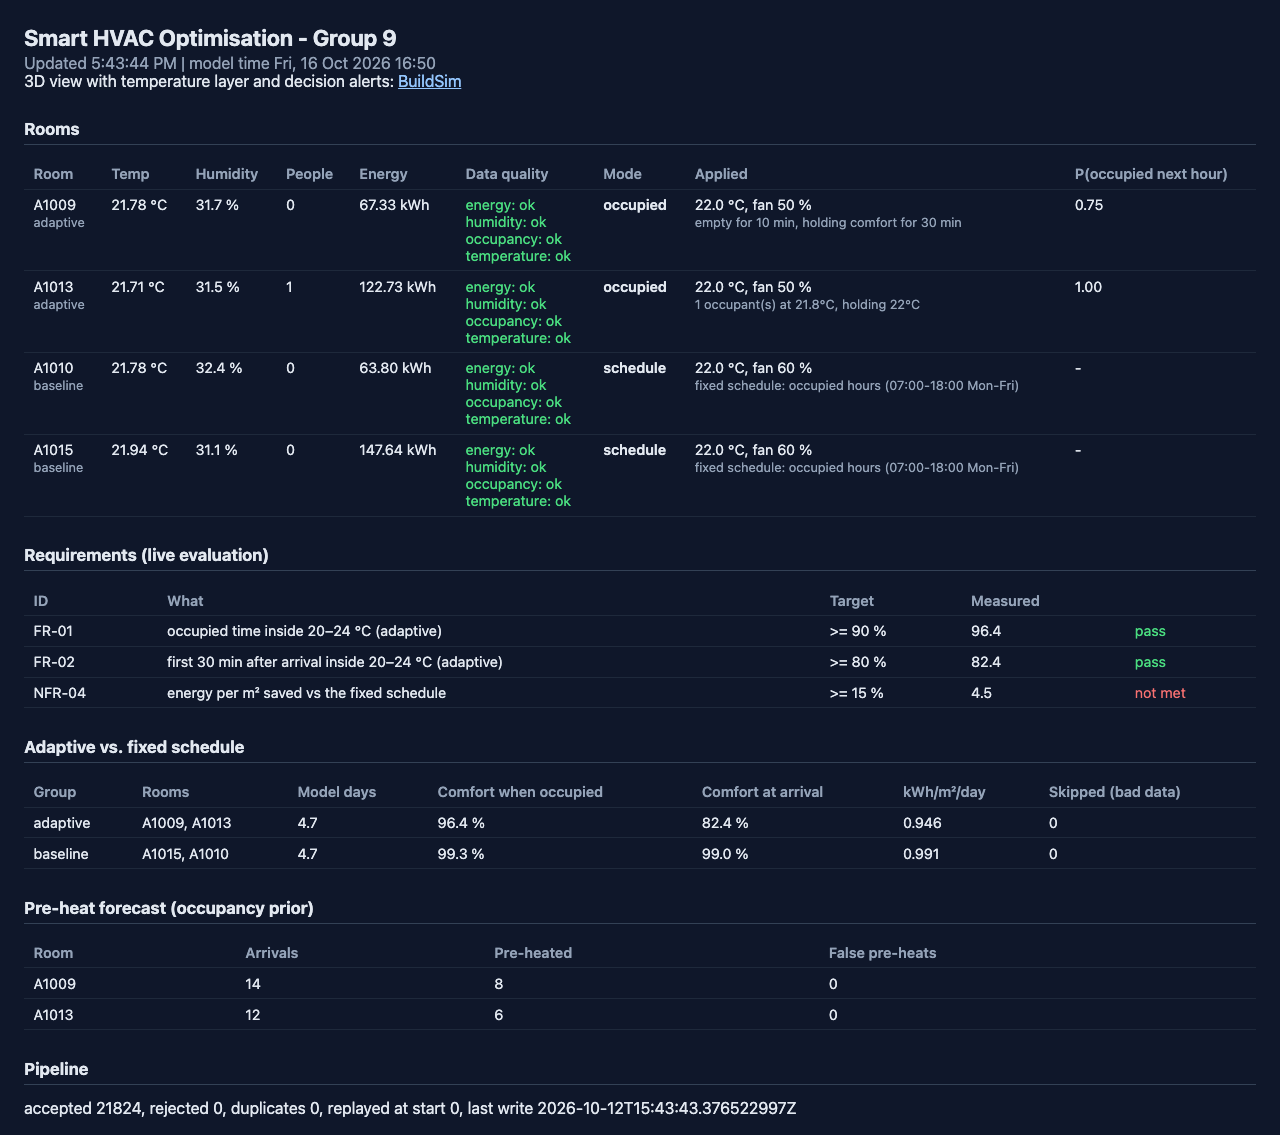
\includegraphics[width=\linewidth]{figures/dashboard.png}\end{minipage}\hfill
\begin{minipage}[c]{0.44\linewidth}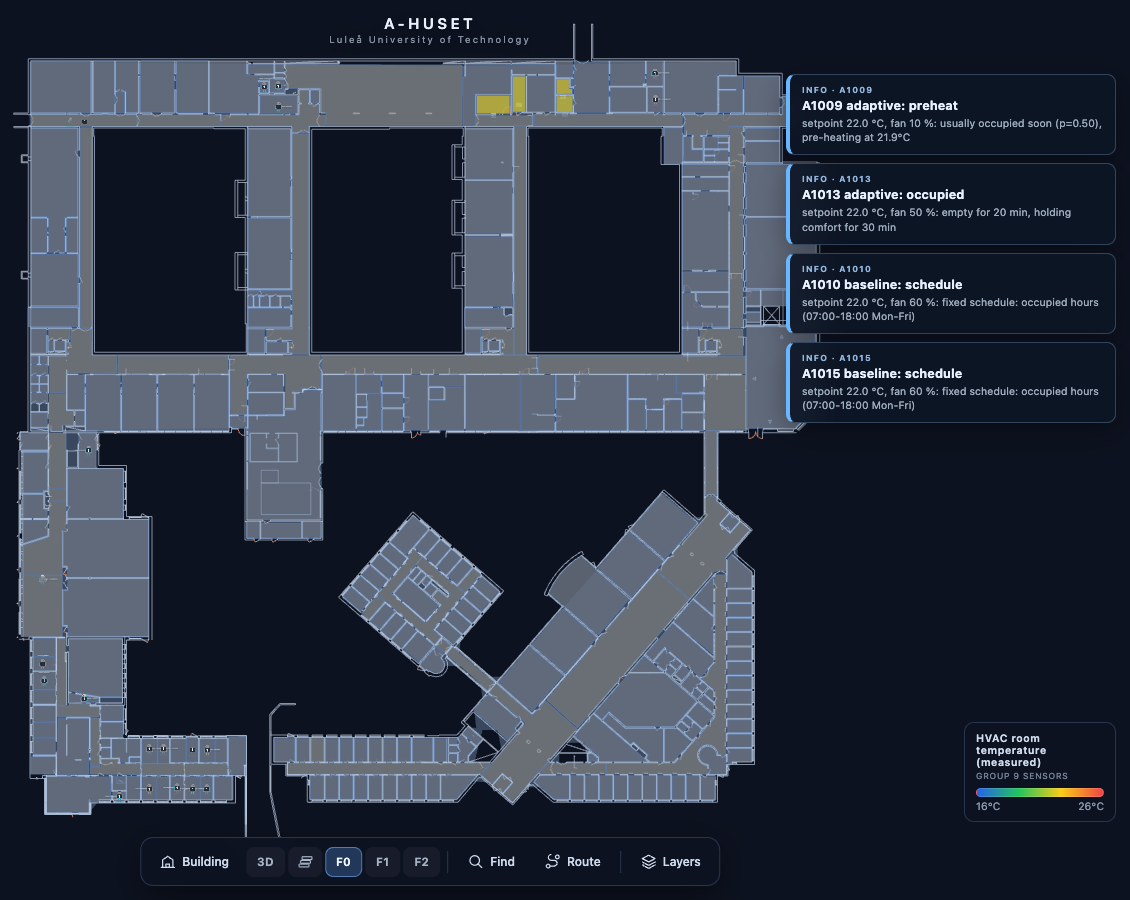
\includegraphics[width=\linewidth]{figures/buildsim_3d.png}\end{minipage}
\end{center}
\figcap{Figure 11. Left: our dashboard, a snapshot taken during the long run (model day 4.7), so its
numbers are not the final ones in Section 11.2. Right: the BuildSim 3D view with our temperature layer
and the decision alerts.}

\section{13. Risks and critical reflection}\label{risks}

We met 11 of our 12 requirements. NFR-04 (15 \% less energy) was not met: we measured 3.6 \%,
because most of the energy is used when both controllers do the same thing (Section 11.5). The
biggest weaknesses are that a slowly drifting sensor is not detected, that night guards make our
rooms heat for nobody, and that every number comes from our own simulation. The honest headline
is ``3.6 \% less than this schedule, in this simulation'', not ``3.6 \% less energy''.

\begin{longtable}{@{}L{0.32}L{0.33}L{0.35}@{}}
\toprule
\textbf{Risk / assumption} & \textbf{Impact} & \textbf{Mitigation / decision} \\
\midrule
\endhead
\bottomrule
\endlastfoot
A sensor drifts slowly (not stuck, not stale) & Wrong decisions on normal-looking data & Compare with the physics or a neighbour room (next step) \\
One clock source (occupancy simulator) & If it is down, services continue the time and occupancy freezes & Accepted: without it there is no occupancy anyway \\
Pipeline or actuator is a single point of failure & All rooms fail safe together, or commands stop & Docker restarts them; sensors buffer; BuildSim keeps the last state \\
Simple physics (no sun, no heat between rooms) & Absolute kWh and comfort are not real-building numbers & Results are reported relative to the baseline \\
Frozen simulator not detected (take-down test) & Values look normal & Accepted for the course \\
Humidity rule never fired in the long run & FR-04 is shown by unit tests only & Test in a room with more people \\
Two copies of our controller share one name & The actuator cannot keep them apart & Give each copy its own source name before sharding \\
\end{longtable}

\textbf{What we would do next:} detect drift; move to MQTT once a second consumer of raw readings
appears; add a slow planning loop that chooses when to start pre-heating from the table and a
weather forecast; and scale the controller out, by deciding rooms in parallel or by running
several controllers, each with its own rooms and source name.

\section{Appendix A: Contribution statement}\label{appendix-a}

We wrote the proposal together and worked out the architecture together: the C4 diagrams and the
design decisions. Monika built the first working version of every service, and the final system is
built on that code. Abhay then tested it against the course requirements and improved it. We both
reviewed the final system and this report.

\begin{longtable}{@{}L{0.2}L{0.4}L{0.4}@{}}
\toprule
\textbf{Area} & \textbf{Monika Shrivastava} & \textbf{Abhay Soni} \\
\midrule
\endhead
\bottomrule
\endlastfoot
Architecture & C4 diagrams and design decisions (together); splitting the system into services and connecting them to BuildSim & C4 diagrams and design decisions (together); the requirements \\
Implementation & First working version of all services and the Docker setup & Improvements to the simulator, controller, pipeline and sensors \\
Testing & Review of the tests and their results & Unit tests, system tests and the stress test \\
Evaluation & First baseline and evaluation services; review of the results & The one-week comparison run and its analysis \\
Report preparation & Proposal; review of this report & Proposal; this report and its figures \\
\end{longtable}

\section{Appendix B: Use of AI tools}\label{appendix-b}

We used Claude, an AI coding assistant, during the project; the course allows this. It helped us
write and change code, tests and scripts, draw the diagrams, and put this report into LaTeX. We
decided what the system should do and which suggestions to keep, we ran all tests and experiments
ourselves, and every number in this report comes from our own measurements in
\texttt{docs/evidence/}. We both understand the code and can explain every part of the system.

\end{document}
